\documentclass{article}

\usepackage[dutch]{babel}
\usepackage[margin=3cm]{geometry}
\usepackage{graphicx}
\usepackage{float}
\usepackage{caption}
\usepackage{hyperref}
\usepackage{amsmath}
\usepackage{wrapfig}
\usepackage[parfill]{parskip}

% fonts
\usepackage[T1]{fontenc}
\usepackage{helvet}
\renewcommand{\familydefault}{\sfdefault}

\graphicspath{{img/}}
 
\newcommand{\bold}[1]{\textbf{#1}}

%Define the listing package
\usepackage{listings} %code highlighter
\usepackage{upquote}
\usepackage{color} %use color
\definecolor{mygreen}{rgb}{0,0.6,0}
\definecolor{mygray}{rgb}{0.5,0.5,0.5}
\definecolor{mymauve}{rgb}{0.58,0,0.82}

\begin{document}

\begin{titlepage}
    \author{Tuur Vanhoutte}
    \title{Security}
\end{titlepage}

\pagenumbering{gobble}
\maketitle
\newpage
\tableofcontents
\newpage

\pagenumbering{arabic}

\section{.NET}

.NET is a free, cross-platform, open source developer platform (*) for building many different types of applications.

* languages + libraries

\begin{figure}[H]
    \centering
    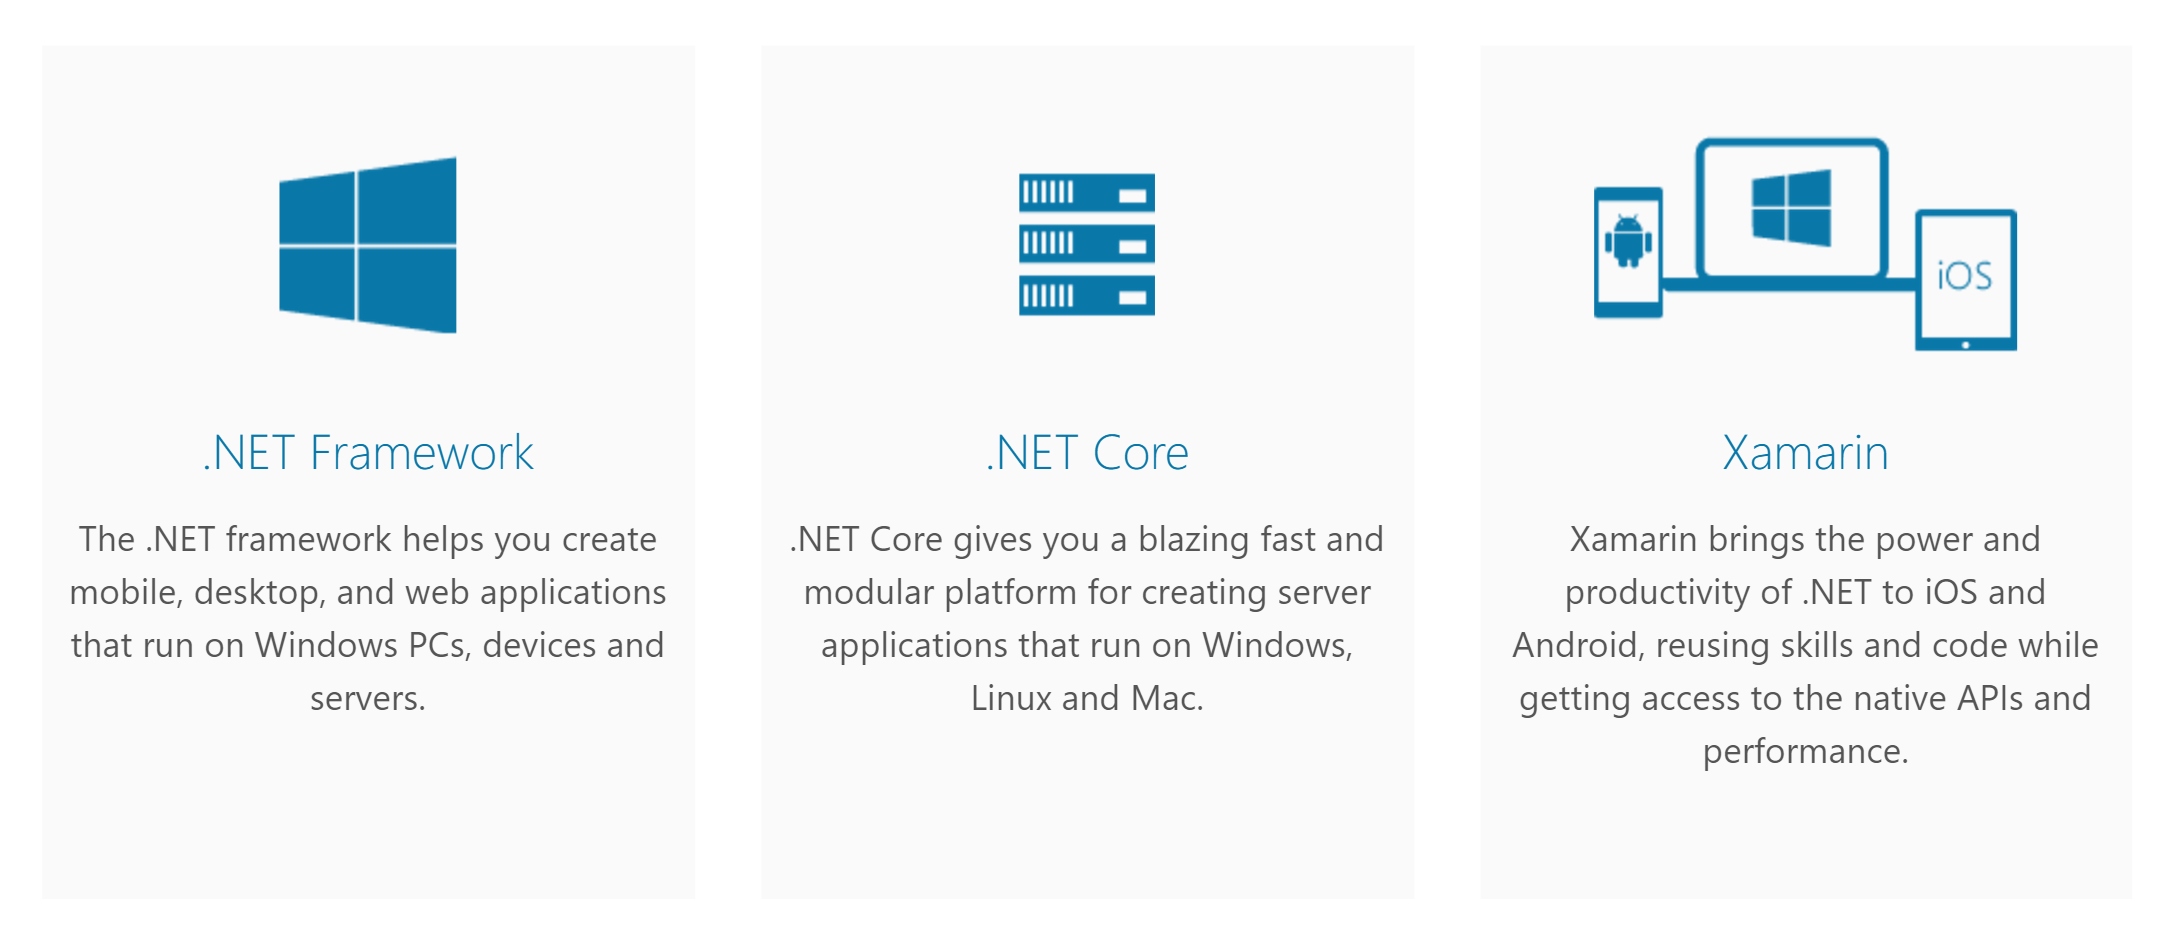
\includegraphics[width=0.8\textwidth]{net-ecosystem.png}
    \caption{.NET ecosystem}
\end{figure}

\subsection{Languages}

\begin{itemize}
    \item Syntax very similar to C, C++, Java \& JavaScript
    \item Functional programming language, cross-platform, open source
    \item Approachable English-like language for OOP
\end{itemize}

\subsection{Applications}

\begin{itemize}
    \item desktop
    \item web \& server
    \item mobile
    \item gaming
    \item IoT
    \item AI
\end{itemize}

\subsubsection{Desktop}

\begin{itemize}
    \item UWP (Universal Windows Project)
    \item Xamarin.Mac
    \item WPF (Windows Presentation Foundation)
    \item WinForms (Windows Forms)
\end{itemize}

\subsubsection{Web \& Server}
\begin{itemize}
    \item ASP.NET
    \item ASP.NET Core
\end{itemize}

\subsubsection{Mobile}
\begin{itemize}
    \item UWP (Universal Windows Project)
    \item Xamarin
\end{itemize}

\subsubsection{Gaming}
\begin{itemize}
    \item Unity
    \item CryEngine
\end{itemize}

\subsubsection{IoT}
\begin{itemize}
    \item UWP
    \item .NET Core IoT
\end{itemize}

\subsubsection{AI}

\begin{itemize}
    \item Cognitive Services
    \item Azure Machine Learning
    \item Machine Learning and AI Libraries
    \item F\# for Data Science and ML
\end{itemize}

\subsection{Xamarin}
\begin{itemize}
    \item `Target all platforms with a single, shared codebase for Android, iOS, Windows'. 
    \item Developen van Mobile devices lastig: verschillende platformen, verschillende talen voor elk device.
    \item Oplossing: Xamarin
    \item Extensie op Visual Studio.
\end{itemize}


\begin{figure}[H]
    \centering
    
\includegraphics[width=0.1\textwidth]{xamarin-logo.png}
    \caption{Xamarin Logo}
\end{figure}

\subsubsection{Xamarin - UI Technology}
\begin{figure}[H]
    \centering
    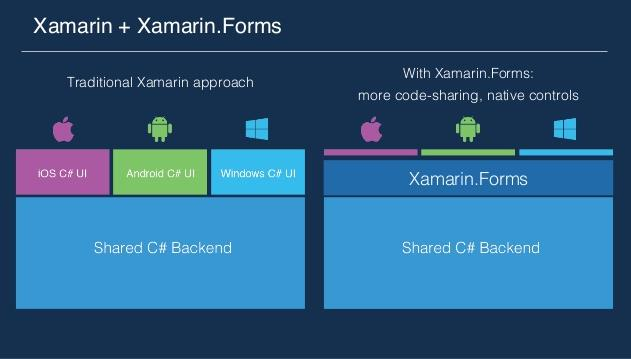
\includegraphics[width=0.7\textwidth]{xamarin-forms.png}
    \caption{Native vs Xamarin.Forms}
\end{figure}

\subsubsection{Xamarin - Code Sharing strategy}

\begin{figure}[H]
    \centering
    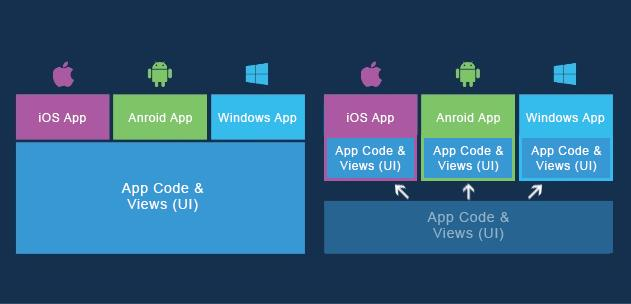
\includegraphics[width=0.7\textwidth]{xamarin-codesharing.png}
    \caption{.NET Standard vs Shared (Assets) Project}
\end{figure}

Met Shared Assets Project maken we de UI voor elk platform apart. Wij gaan vooral werken met .NET Standard.


\subsection{Vragen}

\begin{itemize}
    \item What devices, platforms, etc. can we target using .NET, and what programming languages can we use?
    \item What is the basic difference between .NET Standard and Shared Assets projects in Xamarin?
    \item What is the difference between Xamarin native and Xamarin.Forms? What are the advantages and disadvantages?
    \item How to set up and understand the structure of a Xamarin project for the labs in this course, and how to debug on the different platforms.
\end{itemize}


\end{document}